\chapter{Die Geometrie des homogenen Raums}

\lectureoverview{Die Annahme räumlicher Flachheit beschreibt das beobachtete Universum sehr gut, ist aber kein Prinzip. Wenn wir Homogenität und Isotropie beibehalten, Krümmung jedoch zulassen, ergeben sich drei einfach zusammenhängende räumliche Geometrien: der euklidische, der sphärische und der hyperbolische Raum. Ihre Metriken lassen sich aus dem Wachstum konzentrischer Schalen mit der Entfernung konstruieren; ihre Krümmung lässt sich anhand von Winkelausdehnungen und Objektzahlen prüfen. Auch ein flacher Raum kann endlich sein, wenn seine Topologie torusförmig ist. Schließlich erhält man die Metriken der kosmologischen Raumzeit und das Hubble-Gesetz, wenn man an einen dieser homogenen Räume einen zeitabhängigen Skalenfaktor anfügt; die Dynamik dieses Skalenfaktors muss aus der allgemeinen Relativitätstheorie folgen.}

\section{Flachheit ist eine Beobachtung, kein Prinzip}

Bislang haben wir den Raum als flach behandelt und kaum etwas über die Geometrie der Raumzeit gesagt. Beobachtungen rechtfertigen die Annahme eines flachen Raums als sehr gute Näherung, erheben Flachheit aber nicht zum Gesetz. Die Messungen sagen uns tatsächlich, dass jeder Krümmungsradius groß sein muss im Vergleich zu dem Gebiet, das wir untersucht haben. Der Raum könnte exakt flach, positiv gekrümmt oder negativ gekrümmt sein. Auf Skalen, die weit über das beobachtbare Gebiet hinausgehen, wissen wir noch nicht, welche Beschreibung zutrifft.

Wir lockern daher eine Annahme und behalten eine andere bei. Wir setzen Flachheit nicht voraus, gehen aber weiterhin davon aus, dass der Raum homogen und isotrop ist. Das ist eine Arbeitshypothese, kein Glaubenssatz. Um ihre Folgen zu erkunden, nehmen wir sie an und rechnen; anschließend können wir sie aufgeben und fragen, worin sich ein inhomogenes Universum unterscheiden würde.

Homogenität bedeutet, dass jeder Punkt denselben geometrischen Charakter hat. Ein Beobachter, der sich an einen anderen Ort begibt und dort dieselben lokalen geometrischen Experimente wiederholt, erhält dieselben Ergebnisse. Isotropie bedeutet, dass keine Richtung ausgezeichnet ist. Diese Bedingungen schließen fast alle gekrümmten Flächen aus, die man sich zunächst vorstellt. Ein Paraboloid ist nahe seiner Spitze stärker gekrümmt als weiter entfernt. Ein längliches Ellipsoid unterscheidet sich an seinen Polen und an seinem Äquator. Eine verbeulte Kugel oder die Erdoberfläche, wenn man Berge und Täler auflöst, ist gekrümmt, aber nicht homogen. Die kosmologische Frage ist enger gefasst:
\begin{quote}Welche Räume können gekrümmt sein und dennoch von jedem Punkt aus und in jeder Richtung geometrisch gleich aussehen?
\end{quote}

Lässt man globale Identifizierungen zunächst außer Acht, gibt es drei Antworten mit konstanter Krümmung: den flachen Raum, den positiv gekrümmten sphärischen Raum und den negativ gekrümmten hyperbolischen Raum. Die Einschränkung hinsichtlich globaler Identifizierungen ist wichtig; später werden wir einen endlichen flachen Torus konstruieren und die vereinfachende Aussage korrigieren, diese drei Fälle schöpften alle Möglichkeiten aus.

\section{Die Metrik und die Koordinaten des Beobachters}

Zunächst betrachten wir allein den Raum, nicht die Raumzeit. Seine Geometrie ist in einer Metrik kodiert: einer Vorschrift für das Abstandsquadrat \(ds^2\) zwischen benachbarten Punkten. Sobald diese lokale Vorschrift überall bekannt ist, lassen sich daraus Längen, Winkel, Flächen, Volumina, Geodäten und Krümmung bestimmen.

Für eine euklidische Ebene und den euklidischen dreidimensionalen Raum lauten die Metriken in kartesischen Koordinaten:
\begin{equation}
ds_2^2=dx^2+dy^2,
\qquad
ds_3^2=dx^2+dy^2+dz^2.
\label{eq:c03-cartesian-flat}
\end{equation}
Durch die dritte Dimension kommt lediglich der orthogonale Term \(dz^2\) hinzu; entscheidend ist jedoch nicht die Einfachheit dieser Formel. Entscheidend ist, dass Gleichung~\eqref{eq:c03-cartesian-flat} die lokale Geometrie vollständig festlegt.

\begin{figure}[htbp]\centering
\includegraphics[width=0.74\textwidth]{lecture_03_figure_02.png}\caption{Die kartesische Metrik des flachen dreidimensionalen Raums, wie sie an der Tafel steht.}\label{fig:c03-cartesian-board}\lectureframe{00:05:13.138}\end{figure}

Kartesische Koordinaten geben nicht wieder, wie ein Astronom dem Universum begegnet. Wir befinden uns an einem Punkt, blicken in verschiedene Richtungen nach außen und ordnen das Beobachtete nach Winkel und Entfernung. In einem zweidimensionalen Universum wäre unser Sichtfeld buchstäblich ein Kreis von Richtungen um uns herum. Polarkoordinaten sind daher nicht bloß elegant; sie machen die Winkelgeometrie sichtbar, die in der Kosmologie verwendet wird.

Sei \(r\) der radiale Abstand und \(\theta\) die Richtung. Dieselbe euklidische Ebene hat nun die Metrik
\begin{equation}
ds^2 = dr^2 + r^2 d\theta^2.
\label{eq:c03-polar-flat}
\end{equation}
Bei einem festen kleinen Winkel \(d\theta\) beträgt der transversale Abstand \(r\,d\theta\). Er wächst linear mit der Entfernung vom Ursprung, und sein Beitrag zum Abstandsquadrat ist folglich \(r^2d\theta^2\).

Der Winkelterm ist selbst die Metrik eines eindimensionalen Raums. Ein Kreis ist eine Einersphäre, bezeichnet mit \(S^1\), und die Metrik des Einheitskreises schreibt man üblicherweise als
\begin{equation}
d\Omega_1^2 = d\theta^2,
\qquad\text{so that}\qquad
ds^2 = dr^2 + r^2 d\Omega_1^2.
\label{eq:c03-omega-one}
\end{equation}
An der Tafel steht \(d\Omega^2\) ohne lesbaren Index; aus der mündlichen Definition geht hervor, dass damit \(d\Omega_1^2\) gemeint ist.

\begin{figure}[htbp]\centering
\includegraphics[width=0.74\textwidth]{lecture_03_figure_03.png}\caption{Skizze und Metrik des flachen Raums in Polarkoordinaten. An der Tafel steht \(d\Omega^2\); in der Erläuterung wird dies als Metrik des Einheitskreises identifiziert: \(d\Omega_1^2=d\theta^2\).}\label{fig:c03-polar-board}\lectureframe{00:08:37.254}\end{figure}

\begin{figure}[htbp]\centering
\begin{tikzpicture}[scale=1.2]
\draw[->] (-1.2,0)--(1.8,0);
\draw[->] (0,-1.2)--(0,1.8);
\draw[thick] (0,0)--(1.3,1.1);
\draw (0.7,0.7) node[above] {$r$};
\draw (0.58,0) arc (0:40:0.58);
\draw (0.8,0.22) node {$\theta$};
\end{tikzpicture}\caption{Eine saubere Rekonstruktion der beobachterzentrierten Polarkoordinaten aus Gleichung~\eqref{eq:c03-omega-one}.}\label{fig:c03-polar-redraw}\end{figure}

\begin{classroomqa}\audiencequestion{Misst \(d\theta^2\) tatsächlich den Abstand entlang des Umfangs?}\lecturerresponse{Ja. Auf einem Einheitskreis entspricht die Bogenlänge dem Winkel im Bogenmaß, sodass benachbarte Punkte mit dem Winkelabstand \(d\theta\) einen intrinsischen Abstandsquadraten von \(d\theta^2\) haben. Der Kreis hat den Umfang \(2\pi\), und einmal entlang des Kreises integriert ergibt \(ds=d\theta\) genau \(2\pi\). Mit \(r^2\) multipliziert, wird aus dem Einheitskreis die Schale mit Radius \(r\) in der Ebene. \lecturetimestamp{00:09:11--00:09:26}}\end{classroomqa}

Das Wort \emph{intrinsisch} ist entscheidend. Betten wir den Einheitskreis in eine euklidische Ebene ein, können wir ihn beschreiben durch
\begin{equation}
x^2 + y^2 = 1.
\end{equation}
Diese Gleichung beschreibt, wie der Kreis in einem größeren Raum liegt. Wer nur Abstände entlang des Kreises messen kann, benötigt sie nicht. Wir könnten eine flexible Glasfaser zu einer unregelmäßigen geschlossenen Schleife biegen, ohne sie zu dehnen. Ihr Aussehen in der Ebene änderte sich, aber ihr intrinsischer Umfang und ihre Metrik blieben gleich. Gleiche Zuwächse von \(\theta\) würden weiterhin gleichen Abständen entlang der Faser entsprechen. Die Geometrie muss daher von der zufälligen Gestalt getrennt werden, die eine Einbettung vorgibt.

\begin{figure}[htbp]\centering
\includegraphics[width=0.64\textwidth]{lecture_03_figure_04.png}\caption{An der Tafel werden ein runder Einheitskreis und eine verformte geschlossene Schleife verglichen. Wird die Schleife ohne Dehnung gebogen, haben beide dieselbe intrinsische eindimensionale Metrik.}\label{fig:c03-intrinsic-board}\lectureframe{00:10:34.205}\end{figure}

\begin{figure}[htbp]\centering
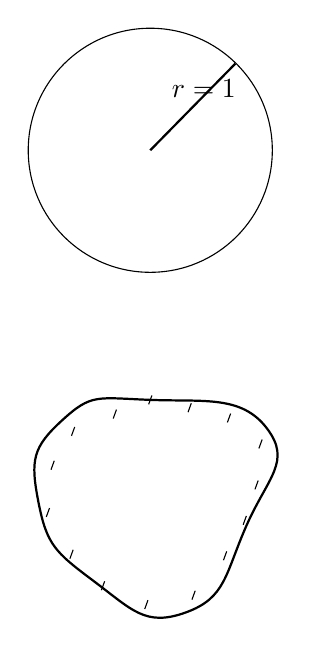
\begin{tikzpicture}[scale=1.0]
\draw (0,0) circle (1.55);
\draw[thick] (0,0)--(1.08,1.1);
\draw (0.68,0.78) node {$r=1$};

\begin{scope}[yshift=-4.35cm]
\draw[thick]
plot[smooth cycle, tension=0.95] coordinates
{(0,1.18) (1.48,0.82) (1.22,-0.42) (0.45,-1.52) (-0.72,-1.12) (-1.42,-0.12) (-1.12,0.92)};
\foreach \p in {(0,1.18),(0.5,1.08),(1.0,0.95),(1.4,0.62),(1.35,0.1),(1.2,-0.35),(0.95,-0.8),(0.55,-1.3),(-0.05,-1.42),(-0.6,-1.18),(-1.0,-0.78),(-1.3,-0.25),(-1.24,0.35),(-0.98,0.78),(-0.45,1.0)}{
\draw[rotate around={70:\p}] \p ++(-0.06,0) -- ++(0.12,0);
}
\end{scope}
\end{tikzpicture}\caption{Der intrinsische Abstand bleibt bei einer extrinsischen Verformung erhalten: Ein eindimensionaler Bewohner misst in beiden Einbettungen denselben Umfang.}\label{fig:c03-intrinsic-redraw}\end{figure}

Der flache Raum lässt sich nun als geschachtelte Familie von Kreisen um den Beobachter auffassen. Die Schale im Abstand \(r\) ist eine mit \(r\) vergrößerte Kopie des Einheitskreises. Genau das bringt der Faktor \(r^2d\Omega_1^2\) zum Ausdruck.

\section{Positive Krümmung: Schalen, die sich schließen}

Eine Kugel ist gekrümmt, aber homogen: Auf einer vollkommen runden Kugel ist kein Punkt geometrisch gegenüber einem anderen ausgezeichnet. Wir können ihre Metrik konstruieren, ohne uns auf ein Bild in einem äußeren dreidimensionalen Raum zu stützen. Stellen wir uns zweidimensionale Astronomen vor, die auf einer Einheits-\(2\)-Sphäre leben und den Ursprung ihres Koordinatensystems an ihrem eigenen Ort wählen.

Der Kreis in ihrem kleinen geodätischen Abstand \(r\) ist klein. Wenn \(r\) zunimmt, wachsen die Kreise, erreichen auf halbem Weg um die Kugel ihren größten Umfang und schrumpfen dann, bis sie am antipodalen Punkt zu einem Punkt zusammenfallen. Dieses Wachstum und Schrumpfen findet mit der \emph{Entfernung} statt, nicht mit der Zeit. Die Kugel ist während dieser gesamten Konstruktion statisch.

Hier ist \(r\) der Winkelabstand entlang der Einheitskugel, nicht der euklidische Abstand von einem Mittelpunkt:
\[
0 \le r \le \pi.
\]
Bei \(r=0\) liegt der gewählte Ursprung, bei \(r=\pi/2\) der Großkreis auf halbem Weg und bei \(r=\pi\) der Antipode. Der Radius der Schale ist nun \(\sin r\), daher wird der flache Faktor \(r^2\) durch \(\sin^2r\) ersetzt:
\begin{equation}
d\Omega_2^2 = dr^2 + \sin^2 r\, d\Omega_1^2
            = dr^2 + \sin^2 r\, d\theta^2.
\label{eq:c03-two-sphere}
\end{equation}
Die Endpunkte und der Mittelpunkt verhalten sich genau wie erforderlich:
\begin{equation}
\sin 0=0,
\qquad
\sin\frac{\pi}{2}=1,
\qquad
\sin\pi=0.
\end{equation}
Die Schalen beginnen also mit verschwindender Größe, erreichen ihre maximale Größe und schließen sich dann wieder.

\begin{figure}[htbp]\centering
\includegraphics[width=0.82\textwidth]{lecture_03_figure_05.png}\caption{Der Übergang von geschachtelten Kreisen im flachen Raum zu Schalen auf der Kugel. Die untere Formel ist im Bild teilweise verdeckt; aus der mündlichen Herleitung ergibt sich der Ersatz \(r^2\mapsto\sin^2r\) in Gleichung~\eqref{eq:c03-two-sphere}.}\label{fig:c03-spherical-board}\lectureframe{00:16:11.701}\end{figure}

\begin{figure}[htbp]\centering
\resizebox{\linewidth}{!}{%
\begin{tikzpicture}[scale=0.92]
\begin{scope}[xshift=-4.15cm]
\draw[->] (-1.7,0)--(1.9,0);
\draw[->] (0,-1.7)--(0,1.9);
\draw (0,0) circle (0.45);
\draw (0,0) circle (0.9);
\draw (0,0) circle (1.35);
\draw[thick] (0,0)--(1.45,1.2);
\draw (0.56,0.18) arc (18:40:0.63);
\draw (0.94,0.44) node {$\theta$};
\end{scope}

\begin{scope}[xshift=4.15cm]
\draw (0,0) circle (2.0);
\fill (0,-2.0) circle (1.5pt);
\fill (2.0,0) circle (1.5pt);
\fill (0,2.0) circle (1.5pt);
\draw[thick] (0,-2.0) arc (-90:90:2.0);
\draw (0,-2.35) node {$r=0$};
\draw (2.75,0) node {$r=\pi/2$};
\draw (0,2.35) node {$r=\pi$};
\end{scope}
\end{tikzpicture}}%
\caption{Flache Schalen wachsen unbegrenzt, während sphärische Schalen bei \(r=\pi/2\) ihre maximale Größe erreichen und sich bei \(r=\pi\) schließen.}\label{fig:c03-shells-flat-sphere}\end{figure}

Die Schreibweise \(d\Omega_2^2\) bezeichnet die Metrik der Einheits-\(2\)-Sphäre, ebenso wie \(d\Omega_1^2\) die Metrik ihrer kreisförmigen Schalen bezeichnet. Dieselbe rekursive Konstruktion funktioniert eine Dimension höher. Bei festem Radius ist die Schale um uns im flachen dreidimensionalen Raum eine \(2\)-Sphäre:
\begin{equation}
ds_{\text{flat},3}^2 = dr^2 + r^2 d\Omega_2^2.
\label{eq:c03-flat-three-polar}
\end{equation}
Wenn diese \(2\)-Sphären mit dem Faktor \(\sin r\) wachsen und sich dann schließen, ergibt sich eine Einheits-\(3\)-Sphäre:
\begin{equation}
d\Omega_3^2 = dr^2 + \sin^2 r\, d\Omega_2^2.
\label{eq:c03-three-sphere}
\end{equation}
Eine \(3\)-Sphäre lässt sich schwer vorstellen, weil ihre vertraute Einbettung vier euklidische Dimensionen erfordern würde. Die Metrik ist jedoch vollständig und benötigt kein Bild. Um einen beliebigen gewählten Beobachter liegen geschachtelte \(2\)-Sphären; sie wachsen bis zu einem Maximum und schrumpfen dann bis zum antipodalen Punkt.

\begin{classroomqa}\audiencequestion{Befindet sich der Beobachter im Mittelpunkt der Kugel?}\lecturerresponse{Der Beobachter befindet sich im Mittelpunkt der \emph{Koordinatenschalen}, nicht in einem ausgezeichneten geometrischen Mittelpunkt. Der Ursprung ist ein Punkt im Raum, und jeder andere Beobachter kann seinen eigenen Ort als \(r=0\) wählen und erhält dieselbe Metrik. Homogenität bedeutet genau, dass keine dieser Wahlen bevorzugt ist. \lecturetimestamp{00:19:21--00:20:27}}\end{classroomqa}

Nur zur Veranschaulichung lassen sich der Einheitskreis und die Einheits-\(2\)-Sphäre in euklidische Räume einbetten:
\begin{equation}
x^2+y^2=1,
\qquad
x^2+y^2+z^2=1.
\end{equation}
Diese Gleichungen beschreiben Einbettungen, keine zusätzliche Physik. Eine Ameise, die auf den Kreis oder die Kugel beschränkt ist, kann die intrinsische Metrik bestimmen, ohne den umgebenden euklidischen Raum nachzuweisen. Ebenso ist \(S^3\) keine gewöhnliche Kugel mit einer rätselhaften Begrenzung. Es ist der vollständige dreidimensionale Raum, der durch Gleichung~\eqref{eq:c03-three-sphere} beschrieben wird.

\section{Wie Krümmung unsere Beobachtungen verändert}

Geometrie wird erst dann zur Physik, wenn sie eine Beobachtung verändert. Angenommen, ein Objekt hat einen bekannten transversalen Durchmesser \(d\), sein radialer Abstand \(r\) wurde unabhängig bestimmt und sein Winkeldurchmesser \(d\theta\) am Himmel gemessen. Galaxien liefern ein grobes, anschauliches Beispiel; in der präziseren Kosmologie verwendet man kalibrierte Standardmaßstäbe und Standardkerzen. Entfernungsinformationen lassen sich aus der spektralen Rotverschiebung, dem Hubble-Zusammenhang, der Leuchtkraft und dem Abgleich verschiedener Objektklassen gewinnen.

Halten wir im flachen Raum über die transversale Breite des Objekts hinweg \(r\) konstant. Gleichung~\eqref{eq:c03-polar-flat} ergibt
\begin{equation}
d^2 = r^2 d\theta^2.
\label{eq:c03-flat-angle-step}
\end{equation}
Daher gilt
\begin{equation}
d\theta = \frac{d}{r}.
\label{eq:c03-flat-angle}
\end{equation}
Der Winkel nimmt umgekehrt proportional zum Abstand ab.

Auf einer Einheitskugel beträgt die transversale Größe der Schale \(\sin r\) statt \(r\):
\begin{equation}
d^2 = \sin^2 r\, d\theta^2,
\qquad\text{hence}\qquad
d\theta = \frac{d}{\sin r}.
\label{eq:c03-spherical-angle}
\end{equation}
Für \(0<r<\pi\) gilt \(\sin r<r\); daher erscheint dasselbe Objekt im selben radialen Abstand größer als im flachen Raum. Seine Winkelausdehnung nimmt zunächst ab, erreicht am Äquator ein Minimum und nimmt dann zu, während sich die Schale zusammenzieht. In der idealisierten Grenzbetrachtung am Antipoden treffen alle Richtungen aufeinander, und das Bild erstreckt sich über den ganzen Himmel.

\begin{classroomqa}\audiencequestion{Ist das dieselbe Idee, mit der sich aus der kosmischen Mikrowellenhintergrundstrahlung die Krümmung bestimmen lässt?}\lecturerresponse{Ja. Das frühe Plasma liefert durch seine akustischen Oszillationen eine charakteristische physikalische Skala. Wir messen den Winkel, unter dem dieser Standardmaßstab erscheint, und vergleichen ihn mit dem von jeder Geometrie vorhergesagten Winkel. Bei den Objekten muss es sich nicht unbedingt um Galaxien handeln; entscheidend ist der Vergleich einer bekannten transversalen Skala mit ihrer beobachteten Winkelausdehnung. \lecturetimestamp{00:37:37--00:38:12}}\end{classroomqa}

Schalenvolumina liefern einen zweiten Test. In drei flachen Dimensionen ist die Fläche einer Schale proportional zu \(r^2\); auf einer Einheits-\(3\)-Sphäre ist sie proportional zu \(\sin^2r\). Eine homogene Population enthält daher auf einer sphärischen Schale zunächst mit zunehmender Entfernung mehr Objekte, nach dem Äquator jedoch weniger. Positive Krümmung sagt gegenüber dem flachen Raum eine charakteristische Kombination zweier Effekte voraus: Standardmaßstäbe in hinreichend großer Entfernung erscheinen zu groß, und hinreichend weit entfernte Schalen enthalten zu wenige Objekte.

\begin{figure}[htbp]\centering
\resizebox{\linewidth}{!}{%
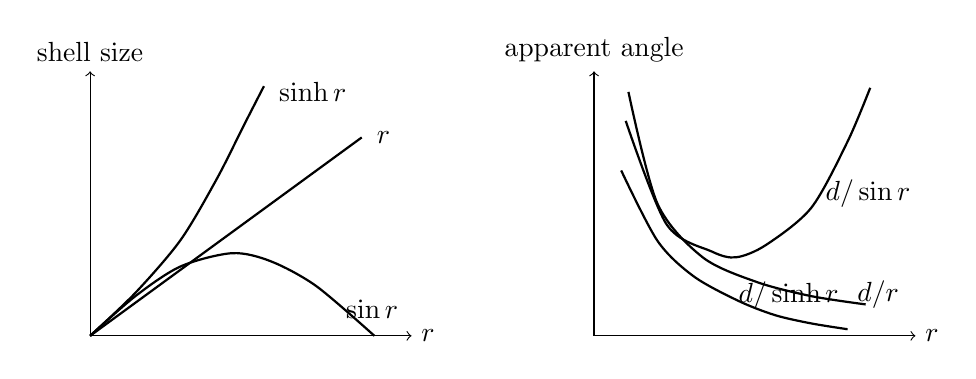
\begin{tikzpicture}[x=1.15cm,y=1.05cm]
\begin{scope}
\draw[->] (0,0)--(3.55,0) node[right] {$r$};
\draw[->] (0,0)--(0,3.2) node[above] {shell size};

\draw[thick] (0,0)--(3.0,2.4);
\draw (3.06,2.4) node[right] {$r$};

\draw[thick]
plot[smooth] coordinates {(0,0) (0.5,0.48) (1.0,0.84) (1.57,1.0) (2.0,0.9) (2.5,0.6) (3.14,0)};
\draw (2.72,0.55) node[below right] {$\sin r$};

\draw[thick]
plot[smooth] coordinates {(0,0) (0.5,0.52) (1.0,1.16) (1.4,1.9) (1.7,2.55) (1.92,3.02)};
\draw (1.98,2.95) node[right] {$\sinh r$};
\end{scope}

\begin{scope}[xshift=6.4cm]
\draw[->] (0,0)--(3.55,0) node[right] {$r$};
\draw[->] (0,0)--(0,3.2) node[above] {apparent angle};

\draw[thick]
plot[smooth] coordinates {(0.38,2.95) (0.7,1.6) (1.2,0.95) (1.8,0.65) (2.4,0.48) (3.0,0.38)};
\draw (2.8,0.5) node[right] {$d/r$};

\draw[thick]
plot[smooth] coordinates {(0.35,2.6) (0.8,1.35) (1.3,1.02) (1.57,0.95) (1.9,1.1) (2.4,1.55) (2.8,2.35) (3.05,3.0)};
\draw (2.45,1.72) node[right] {$d/\sin r$};

\draw[thick]
plot[smooth] coordinates {(0.3,2.0) (0.7,1.15) (1.1,0.72) (1.6,0.42) (2.0,0.25) (2.4,0.15) (2.8,0.08)};
\draw (2.15,0.2) node[above] {$d/\sinh r$};
\end{scope}
\end{tikzpicture}}%
\caption{Radiale Schalenfaktoren und die entsprechenden Winkelausdehnungsgesetze. Bei positiver Krümmung schließt sich die Schale; bei negativer Krümmung wächst sie exponentiell.}\label{fig:c03-shell-angular-laws}\end{figure}

\begin{classroomqa}\audiencequestion{Wird die Radialkoordinate unendlich, wenn wir auf der Kugel immer weitergehen?}\lecturerresponse{Nein. Auf der Einheitskugel ist \(r\) der geodätische Winkelabstand und reicht nur von \(0\) bis \(\pi\). Bei \(r=\pi\) ist die Schale am Antipoden zu einem Punkt zusammengefallen. Hier betrachten wir eine feste räumliche Geometrie und verfolgen kein Objekt durch die Zeit nach außen. Wenn wir später einen Krümmungsradius einführen, werden alle physikalischen Abstände mit diesem Radius multipliziert, doch der dimensionslose Wertebereich ändert sich dadurch nicht. \lecturetimestamp{00:39:30--00:40:35}}\end{classroomqa}

\section{Projektion ist keine Geometrie}

Bevor wir uns der negativen Krümmung zuwenden, lohnt es sich zu sehen, wie stark ein Bild eine geometrisch getreue Darstellung verzerren kann. Setzen wir eine Kugel so auf eine Ebene, dass ihr Südpol die Ebene berührt. Ziehen wir durch jeden Punkt \(P\) der Kugel eine Gerade vom Nordpol aus und verlängern sie bis zur Ebene zum Punkt \(P'\). Das ist die stereografische Projektion. Der Nordpol selbst wird ins Unendliche projiziert. Eine kleine Region nahe dem Südpol wird kaum verzerrt dargestellt, während gleich große intrinsische Regionen nahe dem Nordpol auf der Ebene riesig erscheinen.

Die Verzerrung gehört zur Abbildung, nicht zur Kugel. Die Ausgangskugel bleibt homogen, obwohl ihr ebenes Bild gleichwertigen Regionen sehr unterschiedliche Koordinatengrößen zuweist. Diese Unterscheidung brauchen wir wieder, wenn ein unendlicher hyperbolischer Raum in eine endliche Kreisscheibe abgebildet wird.

\begin{figure}[htbp]\centering
\resizebox{\linewidth}{!}{%
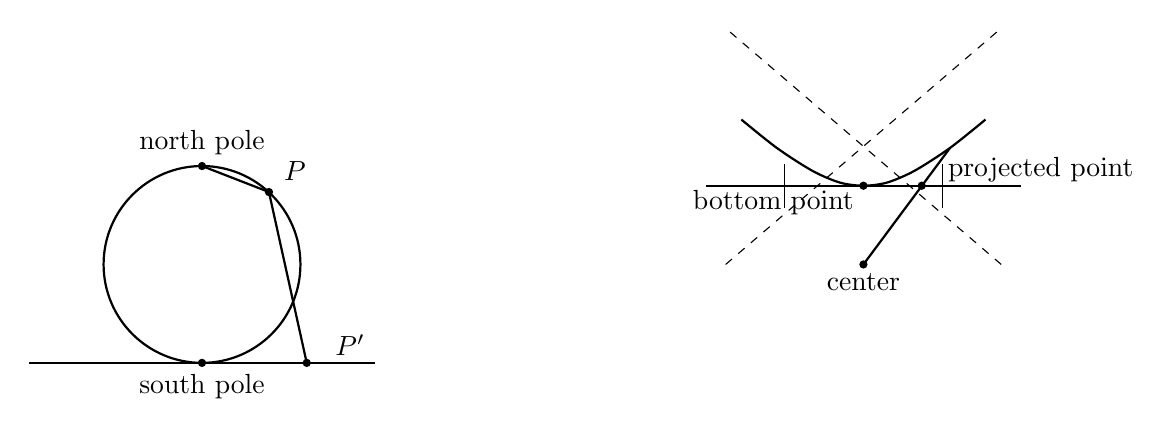
\begin{tikzpicture}[scale=1.0]
\begin{scope}[xshift=-4.2cm]
\draw[thick] (-2.2,-1.25)--(2.2,-1.25);
\draw[thick] (0,0) circle (1.25);
\fill (0,1.25) circle (1.5pt);
\fill (0,-1.25) circle (1.5pt);
\draw (0,1.55) node {north pole};
\draw (0,-1.55) node {south pole};

\fill (0.85,0.92) circle (1.5pt);
\draw (0.92,1.18) node[right] {$P$};
\draw[thick] (0,1.25)--(0.85,0.92)--(1.33,-1.25);
\fill (1.33,-1.25) circle (1.5pt);
\draw (1.57,-1.03) node[right] {$P'$};
\end{scope}

\begin{scope}[xshift=4.2cm]
\draw[thick] (-2.0,1)--(2.0,1);
\draw[dashed] (-1.75,0)--(1.75,3.0);
\draw[dashed] (1.75,0)--(-1.75,3.0);
\draw[thick]
plot[smooth] coordinates
{(-1.55,1.84) (-1.1,1.48) (-0.65,1.19) (-0.3,1.04) (0,1.0) (0.3,1.04) (0.65,1.19) (1.1,1.48) (1.55,1.84)};
\fill (0,0) circle (1.5pt);
\fill (0,1) circle (1.5pt);
\draw (0,-0.22) node {center};
\draw (0,0.78) node[left] {bottom point};
\draw[thick] (0,0)--(1.1,1.48);
\fill (0.74,1.0) circle (1.5pt);
\draw (0.95,1.2) node[right] {projected point};
\draw (-1,0.72) -- (-1,1.28);
\draw (1,0.72) -- (1,1.28);
\end{scope}
\end{tikzpicture}}%
\caption{Links: Bei der stereografischen Projektion wird der Nordpol einer Kugel ins Unendliche projiziert. Rechts: Ein Hyperboloid lässt sich in eine endliche Kreisscheibe projizieren, hier dargestellt durch einen Querschnitt. Die Koordinatenverzerrung hebt die intrinsische Homogenität nicht auf.}\label{fig:c03-projections}\end{figure}

\section{Negative Krümmung: Schalen, die schneller wachsen als im flachen Raum}

In der dritten einfach zusammenhängenden homogenen Geometrie wird \(\sin r\) durch den hyperbolischen Sinus ersetzt. Die Einheitsmetriken in zwei und drei Dimensionen lauten
\begin{equation}
dh_2^2 = dr^2 + \sinh^2 r\, d\Omega_1^2,
\label{eq:c03-hyperbolic-two}
\end{equation}
\begin{equation}
dh_3^2 = dr^2 + \sinh^2 r\, d\Omega_2^2.
\label{eq:c03-hyperbolic-three}
\end{equation}
Die Koordinate \(r\) nimmt nun Werte im Bereich
\begin{equation}
0\le r<\infty.
\end{equation}
an. Nahe dem Ursprung gilt \(\sinh r\approx r\), die Geometrie ist dort also lokal euklidisch. In großer Entfernung wachsen die Schalen viel schneller als euklidische Schalen und kehren niemals um.

Das Wachstumsgesetz folgt aus
\begin{equation}
\sin r = \frac{e^{ir}-e^{-ir}}{2i},
\qquad
\sinh r = \frac{e^r-e^{-r}}{2}.
\label{eq:c03-sin-sinh}
\end{equation}
Für große \(r\) gilt \(\sinh r\sim e^r/2\). In zwei Dimensionen wächst der Umfang daher exponentiell mit dem Radius; in drei Dimensionen wächst die Schalenfläche wie \(\sinh^2r\sim e^{2r}/4\). Eine homogene Verteilung enthält dementsprechend viele Objekte auf einer weit entfernten Schale.

Für ein transversales Objekt der Größe \(d\) gilt
\begin{equation}
d^2 = \sinh^2 r\, d\theta^2,
\qquad\text{so}\qquad
d\theta = \frac{d}{\sinh r}.
\label{eq:c03-hyperbolic-angle}
\end{equation}
Für große \(r\) gilt
\begin{equation}
d\theta \sim 2d\,e^{-r}.
\end{equation}
Negative Krümmung führt somit zum entgegengesetzten Effekt wie positive Krümmung: Standardmaßstäbe in großer Entfernung erscheinen zu klein, während weit entfernte Schalen im Vergleich zum flachen Raum zu viele Objekte enthalten.

\begin{classroomqa}\audiencequestion{Woran unterscheiden sich der radiale Wertebereich auf der Kugel und im hyperbolischen Raum?}\lecturerresponse{Auf der Einheitskugel endet \(r\) am Antipoden bei \(r=\pi\). Im hyperbolischen Raum wächst \(0\le r<\infty\) unbegrenzt weiter. Der Schalenfaktor zeigt denselben Unterschied: \(\sin r\) fällt wieder auf null, während \(\sinh r\) unbegrenzt wächst. \lecturetimestamp{00:52:46--00:53:25}}\end{classroomqa}

Es gibt eine Einbettung, die Homogenität weniger rätselhaft erscheinen lässt. Führen wir Umgebungskoordinaten \(T,x,y\) ein, wobei \(T\) lediglich eine Einbettungskoordinate und \emph{keine} kosmologische Zeit ist, und betrachten wir den oberen Hyperboloidzweig
\begin{equation}
T^2 - x^2 - y^2 = 1.
\label{eq:c03-hyperboloid}
\end{equation}
Statten wir den Umgebungsraum mit der Metrik der Lorentz-Signatur aus:
\begin{equation}
d\ell_{\mathrm{emb}}^2=-dT^2+dx^2+dy^2.
\label{eq:c03-ambient-minkowski}
\end{equation}
Die auf dem Hyperboloid induzierte Metrik ist positiv definit. Lorentz-Transformationen lassen sowohl Gleichung~\eqref{eq:c03-hyperboloid} als auch~\eqref{eq:c03-ambient-minkowski} invariant und können jeden Punkt des oberen Zweigs auf jeden anderen abbilden. In diesem Sinn ist ein Wechsel des Ursprungs im hyperbolischen Raum so, als würde man die Zeitachse im Hilfsraum kippen. Jeder Punkt ist geometrisch gleichwertig.

Projiziert man das Hyperboloid in eine Kreisscheibe, häufen sich die unendlich weit entfernten Punkte am Randkreis. Nahe Regionen werden nahezu unverzerrt dargestellt; weiter entfernte Regionen werden immer stärker zusammengedrückt. Dies ist die Poincar\'e-Scheibendarstellung, die von den Abbildungen mit sich wiederholenden Engeln und Teufeln bekannt ist. Eine Koordinatentransformation kann eine scheinbar winzige Figur nahe dem Rand in die Mitte verschieben, wo sie groß erscheint, und dabei alle intrinsischen Längen und Winkel erhalten. In drei Dimensionen entspricht dem eine Kugel statt einer Kreisscheibe. Die Bezeichnungen \emph{Poincar\'e-Raum}, \emph{Lobatschewski-Raum} und \emph{Raum konstanter negativer Krümmung} meinen dieselbe lokale Geometrie.

\begin{classroomqa}\audiencequestion{Ähnelt die endliche Kreisscheibe einem Penrose-Diagramm?}\lecturerresponse{In dem begrenzten Sinn ist die Darstellung ähnlich, dass ein unendlicher Bereich in einem endlichen Bild dargestellt wird. Hier repräsentiert die Kreisscheibe jedoch allein den Raum, nicht die Raumzeit oder die kausale Unendlichkeit. Ihr Rand ist in der intrinsischen hyperbolischen Metrik unendlich weit entfernt, obwohl er in der Zeichnung bei einem endlichen Koordinatenradius liegt. \lecturetimestamp{01:02:55--01:03:05}}\end{classroomqa}

\section{Der Krümmungsradius}

Die bisher angegebenen Metriken beschreiben Einheitsgeometrien. Um einer Kugel oder einem hyperbolischen Raum einen beliebigen Krümmungsradius zu geben, multiplizieren wir jede Länge mit einer Konstanten. An der Tafel wird diese Konstante mit \(a\) bezeichnet; um sie nicht mit dem später verwendeten zeitabhängigen kosmologischen Skalenfaktor zu verwechseln, nennen wir den statischen Krümmungsradius \(R_c\). Da die Metrik das Längenquadrat misst, gilt
\begin{align}
ds_{\mathrm{sph}}^2
  &=R_c^2d\Omega_n^2
   =R_c^2\left(dr^2+\sin^2r\,d\Omega_{n-1}^2\right),\\
ds_{\mathrm{hyp}}^2
  &=R_c^2dh_n^2
   =R_c^2\left(dr^2+\sinh^2r\,d\Omega_{n-1}^2\right).
\label{eq:c03-scaled-curvature}
\end{align}
Der physikalische radiale Abstand ist \(R_cr\). Ein größerer Wert von \(R_c\) bedeutet geringere Krümmung; der Betrag der konstanten Schnittkrümmung skaliert wie \(1/R_c^2\). Im Grenzfall \(R_c\to\infty\) nähern sich beide gekrümmten Metriken auf jedem festen endlichen Gebiet der euklidischen Geometrie an.

\begin{classroomqa}\audiencequestion{Wird die Kugel weniger oder stärker gekrümmt, wenn sie doppelt so groß wird?}\lecturerresponse{Weniger gekrümmt. Die erste im Unterricht gegebene Antwort wurde durch den Vergleich eines Basketballs mit der Erde korrigiert: Die kleinere Oberfläche krümmt sich über dieselbe Strecke stärker. Eine Verdopplung von \(R_c\) halbiert die Krümmungsskala, die durch den inversen Radius bestimmt ist, und verringert die Schnittkrümmung \(1/R_c^2\) auf ein Viertel. \lecturetimestamp{01:10:14--01:10:56}}\end{classroomqa}

Damit erklärt sich, warum alle drei Geometrien in der unmittelbaren Umgebung gleich aussehen. Für \(r\ll1\) gilt
\begin{equation}
\sin r=r-\frac{r^3}{6}+\cdots,
\qquad
\sinh r=r+\frac{r^3}{6}+\cdots.
\end{equation}
Der führende Term beider gekrümmter Metriken ist die flache polare Metrik; Krümmung tritt erstmals durch Korrekturen relativer Ordnung \((L/R_c)^2\) über eine physikalische Skala \(L\) auf.

\begin{classroomqa}\audiencequestion{Verraten uns die Beobachtungen, ob der Raum flach, sphärisch oder hyperbolisch ist?}\lecturerresponse{Sie zeigen uns, dass das beobachtbare Gebiet sehr nahe an flach ist. Die grobe Schätzung aus dem Unterricht lautete: Eine Schranke von einem Prozent für Krümmungseffekte bedeutet, dass \(R_c\) mindestens ungefähr zehnmal so groß ist wie das sichtbare Gebiet, denn \((L/R_c)^2\lesssim10^{-2}\). Ein entsprechendes Krümmungsvolumen wäre dann mindestens ungefähr \(10^3\) sichtbare Volumina groß. Dies ist eine Abschätzung der Größenordnung aus der Vorlesung, kein Zitat aus aktuellen Präzisionsdaten; exakte Flachheit bleibt die \(R_c=\infty\)-Möglichkeit. \lecturetimestamp{01:11:00--01:13:37}}\end{classroomqa}

\section{Flach, aber endlich: der Torus}

Wir müssen nun die Aussage korrigieren, flache, sphärische und hyperbolische Räume seien die einzigen homogenen Möglichkeiten. Es handelt sich um die drei einfach zusammenhängenden Geometrien konstanter Krümmung. Ein flacher Raum kann außerdem eine nichttriviale globale Topologie haben.

Beginnen wir mit einem euklidischen Rechteck. Identifizieren wir Punkt für Punkt seine linke und rechte Kante und ebenso seine untere und obere Kante. Beim Überschreiten einer Kante gelangt man durch die gegenüberliegende wieder in den Raum. Die lokale Metrik bleibt \(dx^2+dy^2\), aber der globale Raum ist periodisch und endlich. Dieser Quotientenraum ist ein flacher zweidimensionaler Torus \(T^2\). Eine periodische Dimension ergibt einen Kreis \(T^1\); die Identifizierung gegenüberliegender Flächen eines rechteckigen Quaders ergibt einen flachen dreidimensionalen Torus \(T^3\), und die Konstruktion lässt sich auf beliebig viele Dimensionen erweitern.

\begin{figure}[htbp]\centering
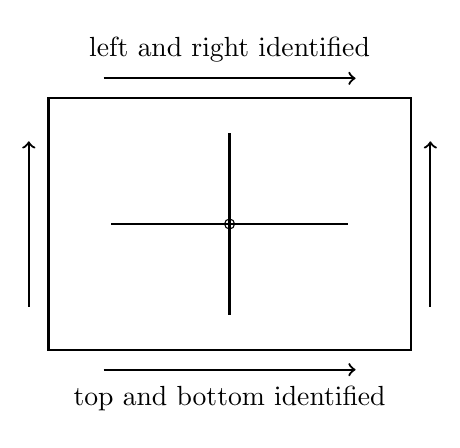
\begin{tikzpicture}[scale=1.0]
\draw[thick] (0,0) rectangle (4.6,3.2);

\draw[->,thick] (0.7,3.45)--(3.9,3.45);
\draw[->,thick] (0.7,-0.25)--(3.9,-0.25);

\draw[->,thick] (-0.25,0.55)--(-0.25,2.65);
\draw[->,thick] (4.85,0.55)--(4.85,2.65);

\draw[thick] (0.8,1.6)--(3.8,1.6);
\draw[thick] (2.3,0.45)--(2.3,2.75);

\draw (2.3,1.6) circle (1.8pt);

\draw (2.3,-0.62) node {top and bottom identified};
\draw (2.3,3.82) node {left and right identified};
\end{tikzpicture}\caption{Ein flacher Torus, konstruiert durch Identifizierung gegenüberliegender Seiten eines Rechtecks. Die Kanten sind keine Ränder; gepaarte Punkte sind im Quotientenraum ein und derselbe Punkt.}\label{fig:c03-flat-torus}\end{figure}

\begin{classroomqa}\audiencequestion{Kann ein Universum demnach zugleich flach und endlich sein?}\lecturerresponse{Ja. Flachheit ist eine lokale Aussage über die Metrik; Endlichkeit kann eine globale Aussage über die Topologie sein. Ein hinreichend großer dreidimensionaler Torus sähe im gesamten beobachtbaren Gebiet euklidisch aus, obwohl sein Gesamtvolumen endlich wäre. \lecturetimestamp{01:13:37--01:17:59}}\end{classroomqa}

Die Darstellung auf der universellen Überlagerung macht die beobachtbare Folge anschaulich. Statt die Kanten zu identifizieren, kacheln wir eine unendliche euklidische Ebene mit Kopien des Fundamentalrechtecks. Ein einzelnes Objekt im Torus erscheint in jeder Kopie einmal. In drei Dimensionen bilden die Kopien ein periodisches, kristallartiges Muster.

\begin{classroomqa}\audiencequestion{Könnten wir in einem torusförmigen Universum leben, ohne es zu bemerken?}\lecturerresponse{Ja, wenn die Fundamentalzelle größer ist als das Gebiet, aus dem Licht uns erreicht hat. Wäre sie klein genug, könnte das Licht die Identifizierungen durchqueren, und wir würden dieselben Galaxien aus verschiedenen Richtungen mehrfach sehen, vielleicht sogar unsere eigene Umgebung wiederholt. Die lokale Geometrie bliebe in beiden Fällen flach. \lecturetimestamp{01:18:16--01:22:04}}\end{classroomqa}

\begin{classroomqa}\audiencequestion{Warum endet die Kugel an ihrem Antipoden, während sich der Torus wiederholt?}\lecturerresponse{Auf der Kugel schrumpft die umgebende Schale tatsächlich bei \(r=\pi\) auf null; alle radialen Richtungen treffen am Antipoden zusammen. Auf einem Torus schrumpft der Rand einer gewählten rechteckigen Zelle nicht. Er wird mit einem gleich großen gegenüberliegenden Rand identifiziert, sodass man beim Überschreiten in einer periodischen Koordinatenbeschreibung im selben Raum weitergeht. \lecturetimestamp{01:22:06--01:23:02}}\end{classroomqa}

\section{Vom Raum zur Raumzeit}

Nun können wir die Zeit wieder einführen. In Einheiten mit Lichtgeschwindigkeit \(c=1\) lautet die Minkowski-Metrik
\begin{equation}
ds^2 = -dt^2 + dx^2 + dy^2 + dz^2.
\label{eq:c03-minkowski}
\end{equation}
Die Vorzeichenkonvention ist eine Wahl; entscheidend ist, dass der Zeitanteil das entgegengesetzte Vorzeichen zu den Raumanteilen hat. Ein Lichtstrahl folgt einer lichtartigen Bahn:
\begin{equation}
ds^2 = 0.
\end{equation}
Für eine Bewegung allein entlang \(x\) gilt
\begin{equation}
-dt^2 + dx^2 = 0
\qquad\Rightarrow\qquad
dx = \pm dt.
\label{eq:c03-null-flat}
\end{equation}
Die beiden Vorzeichen beschreiben Licht, das sich mit Einheitsgeschwindigkeit nach links oder rechts bewegt.

Für die Kosmologie behalten wir den Eigenzeitanteil \(-dt^2\) bei, ersetzen den euklidischen Raumanteil durch eine homogene räumliche Metrik und lassen deren Gesamtskala mit der Zeit variieren. Diesen Skalenfaktor bezeichnen wir mit \(a(t)\). Nun ist er eine dynamische Funktion und nicht mehr der feste Radius \(R_c\), der im vorangegangenen statischen Vergleich verwendet wurde.

Als anschauliches Beispiel in \(2+1\) Dimensionen betrachten wir
\begin{equation}
ds^2 = -dt^2 + a(t)^2 d\Omega_2^2.
\label{eq:c03-two-plus-one}
\end{equation}
Zu jedem festen \(t\) ist der Raum eine \(2\)-Sphäre mit Radius \(a(t)\). Stapelt man diese Sphären in der Zeit, erhält man die Raumzeit. Die vertraute Konstruktion in \(3+1\) Dimensionen lautet
\begin{equation}
ds^2 = -dt^2 + a(t)^2 d\Sigma^2,
\label{eq:c03-frw-general}
\end{equation}
Dabei ist \(d\Sigma^2\) eine zeitunabhängige räumliche Einheitsmetrik. Die drei einfach zusammenhängenden Fälle sind
\begin{align}
\text{flat:}\quad
ds^2&=-dt^2+a(t)^2\left(dx^2+dy^2+dz^2\right),\label{eq:c03-frw-flat}\\
\text{spherical:}\quad
ds^2&=-dt^2+a(t)^2d\Omega_3^2,\label{eq:c03-frw-spherical}\\
\text{hyperbolic:}\quad
ds^2&=-dt^2+a(t)^2dh_3^2.\label{eq:c03-frw-hyperbolic}
\end{align}
Das relative Maß der mitbewegten Koordinaten bleibt fest, während sich \(a(t)\) ändert. Bei der sphärischen und der hyperbolischen Normierung ist \(a(t)\) zugleich der momentane Krümmungsradius. Im flachen Fall kann seine absolute Normierung in den mitbewegten Koordinaten aufgehen.

Das Hubble-Gesetz folgt, bevor irgendeine Gravitationsfeldgleichung angesetzt wird. Betrachten wir zwei nahe beieinanderliegende mitbewegte Punkte mit festem Koordinatenabstand \(\chi\). Ihr physikalischer Abstand ist
\begin{equation}
D(t)=a(t)\chi.
\label{eq:c03-comoving-distance}
\end{equation}
Bei festem \(\chi\) ergibt die Ableitung
\begin{equation}
V=\dot D=\dot a(t)\chi.
\end{equation}
Eliminieren wir \(\chi\), erhalten wir
\begin{equation}
V = \frac{\dot a}{a} D.
\label{eq:c03-hubble-law}
\end{equation}
Somit gilt
\begin{equation}
H = \frac{\dot a}{a}.
\label{eq:c03-hubble-parameter}
\end{equation}
Dies ist eine kinematische Identität für homogene Expansion oder Kontraktion. Sie gilt für alle drei räumlichen Geometrien: Für \(\dot a>0\) entfernen sich die Punkte voneinander, für \(\dot a<0\) nähern sie sich.

Die Geometrie allein legt \(a(t)\) nicht fest. Funktionen wie
\begin{equation}
a(t)\propto t^{2/3},
\qquad
a(t)\propto t^{1/2},
\qquad
a(t)\propto e^{Ht}
\end{equation}
erfüllen alle den homogenen metrischen Ansatz, beschreiben aber unterschiedliche kosmische Materie- und Energieinhalte. Die Allgemeine Relativitätstheorie liefert die dynamische Gleichung, die zwischen ihnen entscheidet. Die daraus folgende Friedmann-Gleichung wird außerdem die flachen, sphärischen und hyperbolischen Fälle mit den Alternativen verschwindender, negativer und positiver Energie der zuvor entwickelten Newtonschen Kosmologie verbinden.

\begin{classroomqa}
\audiencequestion{Könnten die Geometrie und die kosmische Entwicklung viel komplizierter sein als in diesen Modellen?}
\lecturerresponse{Gewiss. Homogenität und Isotropie sind einschränkende Annahmen. Sie werden gewählt, weil sie naheliegen, auf großen Skalen mit den Beobachtungen übereinstimmen und mathematisch handhabbar sind. Es gibt zahlreiche kompliziertere Geometrien und Entwicklungsverläufe. Eine wichtige dynamische Frage ist, ob sich große Klassen anfangs unregelmäßiger Modelle zu einer dieser einfachen homogenen Formen entwickeln. \lecturetimestamp{01:36:00--01:36:50}}
\end{classroomqa}

\begin{classroomqa}
\audiencequestion{Ist die \(3\)-Sphäre der Rand eines vierdimensionalen Objekts?}
\lecturerresponse{Als Einbettung lässt sie sich so darstellen, doch der kosmologische Raum ist die \(3\)-Sphäre selbst. Sie hat drei intrinsische Dimensionen und keinen Rand. Die vierdimensionale euklidische Darstellung ist lediglich ein optionales Hilfsmittel; Gleichung~\eqref{eq:c03-three-sphere} legt die Geometrie bereits vollständig fest. \lecturetimestamp{01:36:55--01:37:59}}
\end{classroomqa}

\begin{classroomqa}
\audiencequestion{Ist die Leuchtkraft der einzige Weg, um die für den Krümmungstest benötigte Entfernung zu bestimmen?}
\lecturerresponse{Nein. Spektrallinien bestimmen die Rotverschiebung, nahe Entfernungsleitern kalibrieren die Hubble-Beziehung, und Supernovae liefern näherungsweise Standardleuchtkräfte. Diese Methoden werden miteinander abgeglichen, statt einzeln als verlässlich vorausgesetzt zu werden. Selbst das invers-quadratische Leuchtkraftgesetz hängt von der Geometrie ab, denn die Fläche einer Lichtfront wird durch \(r^2\), \(\sin^2r\) oder \(\sinh^2r\) bestimmt. Die Übereinstimmung mehrerer Messgrößen stützt die Annahme einer nahezu flachen Geometrie. \lecturetimestamp{01:38:00--01:41:07}}
\end{classroomqa}

\section{Was Sie mitnehmen sollten}

Die Geometrie eines homogenen Universums lässt sich daran ablesen, wie Schalen um einen beliebigen Beobachter wachsen:
\begin{equation}
f(r)=
\begin{cases}
r, & \text{flat space},\\
\sin r, & \text{positive curvature},\\
\sinh r, & \text{negative curvature}.
\end{cases}
\end{equation}
Die räumliche Metrik lautet \(dr^2+f(r)^2d\Omega_{n-1}^2\). Dieselbe Funktion bestimmt die Winkelgrößen und die Zahl der Objekte auf einer Schale, sodass die Krümmung unmittelbar beobachtbar ist. Ein großer Krümmungsradius lässt diese Unterschiede lokal kaum erkennen, und eine toroidale Identifikation zeigt, dass die lokale Krümmung für sich genommen weder die globale Größe noch die Topologie festlegt.

Durch Ergänzung um \(-dt^2\) und den gemeinsamen Faktor \(a(t)^2\) wird jede der drei homogenen räumlichen Metriken zu einer kosmologischen Raumzeit. Daraus folgt unmittelbar \(V=HD\) mit \(H=\dot a/a\), doch \(a(t)\) bleibt unbestimmt. Der nächste Schritt ist daher keine weitere geometrische Übung, sondern das dynamische Problem: Mit Einsteins Gleichungen ist zu bestimmen, wie Materie, Strahlung, Krümmung und andere Energieformen die Entwicklung des Skalenfaktors bewirken.
